% Contenido exportado del Word validado; regenerar con exportar_latex.py.

\section*{Presentación del ejercicio}
\phantomsection\addcontentsline{toc}{section}{Presentación del ejercicio}

Este documento desarrolla la Tarea 6 de Seminario I mediante la aplicación de formato APA y un índice automatizado al archivo \emph{Material para ejemplo}. Se conserva su función de guía para organizar un trabajo de titulación: las descripciones de resultados, conclusiones y anexos son orientaciones, no evidencias de una investigación realizada.

La portada institucional se utiliza exclusivamente como ejemplo académico. La designación de la Dra. Carla Olimpya Zapuche Moreno como directora de tesis responde a la consigna y no constituye un nombramiento formal. La estructura capitular procede del material del curso (\emph{Material para ejemplo}, s. f.).

El formato general sigue el \emph{Resumen del Manual APA (7.ª edición)} (s. f.). Se conserva la numeración institucional de capítulos y apartados; las Tablas 1 y 2 y las Figuras 1 y 2 se integran en el marco metodológico con sus fuentes y atribuciones.

\section*{Portada}
\phantomsection\addcontentsline{toc}{section}{Portada}

Debe contener los datos institucionales (nombre del TecNM y del Instituto, logotipo, título del trabajo, nombre del autor, nombre del asesor, grado académico, ciudad y fecha).

\section*{Dedicatoria (opcional)}
\phantomsection\addcontentsline{toc}{section}{Dedicatoria (opcional)}

Espacio personal donde el autor expresa agradecimientos o dedicatorias a personas significativas.

\section*{Agradecimientos (opcional)}
\phantomsection\addcontentsline{toc}{section}{Agradecimientos (opcional)}

Texto breve en el que se reconoce la colaboración de instituciones, asesores, tutores, familiares o colegas que contribuyeron al desarrollo del trabajo.

\section*{Resumen}
\phantomsection\addcontentsline{toc}{section}{Resumen}

Síntesis del contenido de la investigación, que expone de manera breve los objetivos, metodología, resultados y conclusiones más relevantes. Su extensión no debe superar una cuartilla.

\section*{Palabras clave}
\phantomsection\addcontentsline{toc}{section}{Palabras clave}

De tres a cinco términos que representen los conceptos centrales del estudio, permitiendo su indexación temática.

\section*{Índice}
\phantomsection\addcontentsline{toc}{section}{Índice}

Presenta la estructura general del documento con los capítulos, apartados y subapartados, junto con su numeración correspondiente.

\clearpage\section{Introducción}

Presenta el propósito general de la investigación, su justificación y los fundamentos teóricos que la sustentan. Es la carta de presentación del proyecto.

\subsection{Antecedentes o estado del arte}

Describe el origen del tema, los estudios previos y las tendencias actuales relacionadas con la problemática. Incluye información del contexto institucional, social o económico que da sentido al trabajo.

\subsubsection{Contexto del trabajo de titulación}

Expone el ámbito o sector donde se desarrollará la investigación, señalando las características del entorno, la institución o la organización que sirve de base al estudio.

\subsection{Planteamiento del problema}

Identifica la problemática o área de oportunidad. Incluye su diagnóstico, las causas y consecuencias, así como la delimitación temporal, espacial y conceptual. Debe concluir con la pregunta de investigación principal y, si aplica, las preguntas específicas derivadas de los objetivos.

\subsection{Objetivos}

Definen lo que se pretende lograr con la investigación.

\subsubsection{Objetivo general}

Describe la finalidad principal y debe responder a la pregunta de investigación.

\subsubsection{Objetivos específicos}

Desglosan metas concretas que contribuyen al logro del objetivo general. Cada uno puede corresponder a un capítulo o etapa del proyecto.

\subsection{Justificación}

Explica los motivos y la relevancia del estudio, respondiendo a las preguntas: ¿Por qué es importante el tema?, ¿Para qué servirá?, ¿A quién beneficia? Debe vincularse con necesidades reales o vacíos de conocimiento.

\subsection{Alcances y limitaciones}

Define los márgenes y restricciones del estudio.

\subsubsection{Alcances}

Señalan el grado de profundidad del estudio, el periodo, población y variables consideradas.

\subsubsection{Limitaciones}

Describen los factores o condiciones que podrían afectar el desarrollo de la investigación, como tiempo, acceso a información o recursos.

\clearpage\section{Marco teórico}

Sustenta teóricamente la investigación, describiendo conceptos, enfoques, leyes o antecedentes que permiten comprender el fenómeno de estudio.

\subsection{Marco referencial}

El marco referencial constituye el fundamento teórico que permite situar la investigación dentro del conocimiento existente. Su propósito es contextualizar el problema mediante la revisión de antecedentes empíricos, conceptuales e institucionales que sustenten la pertinencia del estudio. Según el material didáctico de Seminario I (\emph{Material para ejemplo}, s. f.), el marco referencial describe las relaciones teóricas entre factores relevantes, facilitando la comprensión del fenómeno y la delimitación de las variables involucradas.

\subsubsection{Antecedentes históricos e institucionales}

En este apartado se presenta la evolución del tema o fenómeno objeto de estudio, desde su surgimiento hasta su situación actual. Incluye hechos, políticas, procesos o decisiones que han influido en su desarrollo, así como la descripción de la institución, sector o entorno donde se origina el problema.

Debe mostrar una línea temporal que refleje los principales hitos, cambios o innovaciones, destacando su relevancia para la investigación. En el caso de proyectos profesionalizantes, se enfatiza la trayectoria del área o unidad organizacional en la que se plantea la mejora o propuesta de intervención.

\subsubsection{Antecedentes teóricos y empíricos}

Aquí se analizan los estudios previos, investigaciones o experiencias que abordan problemáticas similares. Se identifican los enfoques teóricos utilizados, las metodologías aplicadas y los resultados obtenidos, con el fin de reconocer vacíos de conocimiento o áreas poco exploradas.

Se recomienda organizar los antecedentes de lo general a lo particular, iniciando con contextos internacionales, continuando con el ámbito nacional y finalizando con el local o institucional.

Este análisis permite justificar la relevancia del estudio y demostrar la evolución del conocimiento en torno al tema, así como establecer la posición teórica del investigador frente a las evidencias revisadas.

\subsubsubsection{Revisión internacional}

Incluye estudios, modelos o políticas implementadas en otros países que abordan la problemática desde diferentes perspectivas. Este análisis ofrece una visión comparada y permite identificar tendencias globales, enfoques metodológicos y aportaciones teóricas relevantes.

\subsubsubsection{Revisión nacional}

Presenta investigaciones y documentos elaborados en el contexto nacional que guarden relación con el tema. Permite identificar la manera en que la problemática se manifiesta en el país y cómo las políticas públicas, marcos normativos o programas institucionales la han abordado.

\subsubsubsection{Revisión local o institucional}

Describe la información más cercana al ámbito en que se desarrolla la investigación: municipio, región, empresa o institución. Incluye datos estadísticos, diagnósticos, informes internos o registros administrativos que evidencien la situación específica del problema en el entorno inmediato.

\subsubsection{Aportes y vacíos del conocimiento}

Este subapartado sintetiza los principales hallazgos teóricos y empíricos derivados de la revisión, destacando coincidencias, diferencias y vacíos. Permite identificar qué aspectos del fenómeno ya han sido estudiados, qué enfoques teóricos prevalecen y qué dimensiones aún requieren análisis o actualización.

Su propósito es justificar la necesidad y la pertinencia de la investigación, así como sustentar el aporte original que se pretende realizar con el estudio.

\subsection{Marco conceptual}

El marco conceptual constituye la base teórica y semántica del estudio, ya que define los conceptos esenciales, las categorías de análisis y las relaciones entre las variables que integran la investigación. Su propósito es establecer un lenguaje común que oriente la interpretación del fenómeno estudiado y facilite la coherencia entre los objetivos, la metodología y el análisis de resultados.

De acuerdo con el material didáctico de Seminario I (\emph{Material para ejemplo}, s. f.), el marco conceptual debe representar el sistema de ideas que da sentido al problema de investigación y permite articular los conocimientos existentes con la propuesta teórica que el investigador adopta. En este sentido, las definiciones deben provenir de fuentes confiables, actualizadas y académicamente reconocidas.

\subsubsection{Conceptos fundamentales del estudio}

En este apartado se presentan los términos esenciales que sustentan el desarrollo del tema de investigación. Cada concepto debe definirse con claridad, precisión y sustento bibliográfico, utilizando autores que representen diferentes corrientes o perspectivas teóricas.

\subsubsubsection{Definiciones generales}

Incluye los conceptos de carácter amplio y transversal que enmarcan la temática, tales como los vinculados al campo disciplinar (por ejemplo, “gestión”, “innovación”, “eficiencia organizacional”, “política pública”, entre otros). Las definiciones deben establecer la base teórica común del estudio.

\subsubsubsection{Definiciones específicas del problema de investigación}

Se abordan los conceptos que guardan relación directa con las variables o dimensiones centrales del estudio. Este nivel debe ser más analítico, describiendo los términos de manera contextualizada al entorno o institución donde se realiza la investigación.

\subsubsubsection{Definiciones operacionales}

Aquí se definen los conceptos en términos observables y medibles, con base en los indicadores o categorías que se utilizarán en el análisis empírico. Esta sección vincula la teoría con la metodología, facilitando la elaboración de instrumentos de recolección de datos.

\subsubsection{Categorías teóricas y analíticas}

Las categorías teóricas representan los ejes de interpretación que guían el análisis del fenómeno. Estas se derivan de la revisión bibliográfica y expresan los enfoques o modelos teóricos adoptados.

Por su parte, las categorías analíticas corresponden a las dimensiones que permitirán observar el fenómeno en la realidad, facilitando la operacionalización de variables.

\subsubsubsection{Categorías teóricas}

Describe los enfoques conceptuales o modelos que sustentan la investigación (por ejemplo, teoría de sistemas, gestión del cambio, desarrollo organizacional, sostenibilidad, entre otros). Estas categorías deben fundamentarse en autores clave y servir de base interpretativa.

\subsubsubsection{Categorías analíticas o dimensiones de estudio}

Identifica los componentes o dimensiones del fenómeno que serán observadas y medidas. Cada categoría analítica debe relacionarse con una variable o indicador dentro del diseño metodológico.

\subsubsubsection{Relaciones entre categorías y variables}

Explica cómo las categorías teóricas y analíticas se vinculan entre sí, representando un modelo conceptual del problema. Puede apoyarse en esquemas o diagramas conceptuales que muestren las interacciones principales.

\subsubsection{Modelo conceptual del estudio}

El modelo conceptual sintetiza la estructura teórica de la investigación, mostrando las relaciones entre las variables principales y sus posibles efectos o correlaciones. Según el material didáctico de Seminario I (\emph{Material para ejemplo}, s. f.), este modelo funciona como un mapa teórico que orienta la aplicación metodológica y el análisis de resultados.

\subsubsubsection{Identificación de variables}

Se señalan las variables dependientes e independientes, así como las variables intervinientes o de control. Cada una debe definirse claramente en función del marco teórico.

\subsubsubsection{Representación gráfica del modelo conceptual}

Se recomienda incorporar un diagrama o esquema donde se visualicen las relaciones entre las variables, destacando los flujos causales o de correlación que guían la investigación.

\subsubsubsection{Hipótesis derivadas del modelo conceptual}

Se formulan proposiciones contrastables sobre las relaciones entre variables; su comprobación requiere un diseño congruente y evidencia empírica (Conerly et al., 2021).

\subsection{Marco legal}

El marco legal constituye el conjunto de disposiciones normativas, reglamentarias y jurídicas que enmarcan la investigación. Su finalidad es sustentar legalmente el tema, los objetivos y las acciones propuestas, garantizando que el estudio se desarrolle dentro de los límites establecidos por la legislación vigente.

El material didáctico de Seminario I señala que el marco legal permite delimitar las normas que regulan los procesos, las actividades y los sujetos relacionados con el problema, así como las competencias y responsabilidades institucionales (\emph{Material para ejemplo}, s. f.). Su organización parte del ámbito internacional, continúa con el nacional y concluye con la regulación estatal, institucional o sectorial aplicable.

\subsubsection{Fundamento jurídico internacional}

Incluye los tratados, convenios, declaraciones y acuerdos internacionales que se relacionan con la temática de estudio. Estos documentos suelen establecer principios rectores o compromisos adoptados por el Estado mexicano en materia de derechos humanos, desarrollo sostenible, innovación, educación, medio ambiente, género, entre otros.

\subsubsubsection{Tratados y convenciones internacionales}

Se mencionan los principales instrumentos internacionales relacionados con México que inciden en el tema de la investigación, como la Declaración Universal de los Derechos Humanos (Organización de las Naciones Unidas [ONU], 1948), la Agenda 2030 para el Desarrollo Sostenible (ONU, 2015), o los acuerdos internacionales en materia económica, tecnológica o ambiental, según corresponda al objeto de estudio. Las declaraciones y agendas no deben confundirse con tratados sujetos a ratificación.

\subsubsubsection{Organismos internacionales competentes}

Se describen las instituciones globales que impulsan políticas o lineamientos relacionados con el tema, tales como la Organización de las Naciones Unidas (ONU), la Organización Internacional del Trabajo (OIT), la UNESCO, la Organización Mundial del Comercio (OMC) o el Banco Interamericano de Desarrollo (BID).

\subsubsubsection{Aplicabilidad en el contexto nacional}

Analiza cómo los compromisos internacionales asumidos por México se traducen en políticas públicas, reformas normativas o programas nacionales. Este apartado sirve de puente entre el ámbito internacional y el marco jurídico mexicano.

\subsubsection{Fundamento jurídico nacional}

Comprende las leyes, reglamentos, normas oficiales mexicanas y políticas públicas nacionales que sustentan la investigación. Debe establecer el marco jurídico de referencia, destacando las disposiciones que regulan el objeto del estudio y las competencias de las instituciones involucradas.

\subsubsubsection{Constitución Política de los Estados Unidos Mexicanos}

Se identifican los artículos constitucionales relacionados con el tema de investigación. Por ejemplo, el artículo 25 (desarrollo económico y social), el 27 (propiedad de recursos naturales), el 123 (derechos laborales), o el 4 (medio ambiente y salud), según la naturaleza del proyecto.

\subsubsubsection{Leyes, reglamentos y normas complementarias}

Se describen las leyes federales y estatales aplicables (como la Ley General de Educación Superior, la Ley de Ciencia y Tecnología, la Ley General del Equilibrio Ecológico y Protección al Ambiente, entre otras), así como sus reglamentos, normas técnicas o disposiciones secundarias que inciden en el campo de estudio. Las denominaciones legales se conservan como ejemplos del material; su vigencia debe corroborarse en las fuentes jurídicas oficiales antes de aplicarlas a una tesis.

\subsubsubsection{Políticas públicas y programas nacionales}

Aquí se incluyen los programas sectoriales, estrategias nacionales o políticas públicas que orientan las acciones institucionales vinculadas con la temática, tales como el Programa Sectorial de Educación 2020–2024 o el Plan Nacional de Desarrollo 2019–2024. Los periodos 2019–2024 y 2020–2024 se conservan como ejemplos históricos del material base; para una investigación actual deben verificarse los instrumentos vigentes.

\subsubsection{Fundamento jurídico estatal e institucional}

Este nivel delimita la aplicación de la normativa al ámbito territorial o institucional donde se desarrollará la investigación, permitiendo contextualizar las disposiciones federales en el marco local o interno de la organización.

\subsubsubsection{Legislación estatal}

Incluye las leyes, reglamentos y decretos emitidos por el Congreso local o el Gobierno del Estado en relación con el tema de estudio. Por ejemplo, la Ley de Educación del Estado de Sonora, la Ley de Responsabilidad Ambiental del Estado o la Ley de Ciencia y Tecnología de Sonora, según el caso.

\subsubsubsection{Normatividad institucional o sectorial}

Se presentan los reglamentos, lineamientos, manuales y disposiciones internas que regulan el funcionamiento de la institución donde se desarrolla el proyecto. En el caso del TecNM, pueden citarse el Reglamento de Estudios de Posgrado, el Manual de Procedimientos Académicos, o los Códigos de Ética Institucional.

\subsubsubsection{Vinculación entre los niveles normativos}

Finalmente, se analiza la coherencia y correspondencia entre los tres niveles (internacional, nacional e institucional), mostrando cómo se articulan para respaldar la pertinencia legal de la investigación. Este análisis puede complementarse con un esquema o cuadro comparativo que sintetice las normas aplicables y su relación con los objetivos del estudio.

\clearpage\section{Marco metodológico}

Describe el procedimiento seguido para realizar la investigación, explicando el tipo de estudio, las técnicas empleadas y los instrumentos de recolección de información.

\subsection{Tipo de investigación en ciencias sociales}

Especifica si la investigación es cuantitativa, cualitativa o mixta, y el nivel de alcance (exploratoria, descriptiva, correlacional o explicativa).

La Tabla 1 compara métodos de investigación social y ayuda a seleccionar una estrategia congruente con el problema, los objetivos y los recursos disponibles (Conerly et al., 2021). Un método de recolección no debe confundirse con el alcance del estudio.

\begin{table}[H]
\begin{minipage}{\linewidth}
\caption{Métodos de investigación social: técnicas, ventajas y limitaciones}\label{tab:tarea6-1}
\begin{singlespace}
\small\setlength{\tabcolsep}{4pt}
\setlength{\RaggedRightParindent}{0pt}\setlength{\parindent}{0pt}
\renewcommand{\arraystretch}{1.25}
\begin{tabularx}{\linewidth}{@{}>{\RaggedRight\arraybackslash}p{0.14\linewidth}>{\RaggedRight\arraybackslash}p{0.22\linewidth}ZZ@{}}
\toprule
\textbf{Método} & \textbf{Técnicas o fuentes} & \textbf{Ventajas} & \textbf{Limitaciones} \\
\midrule
Encuesta & Cuestionarios y entrevistas & Permite obtener numerosas respuestas y organizar datos cuantitativos. & La participación puede ser baja; lo declarado no siempre coincide con la conducta. \\
Trabajo de campo & Observación participante, etnografía y estudio de caso & Aporta información detallada en contextos reales. & Requiere tiempo; los datos cualitativos demandan organización e interpretación. \\
Experimento & Manipulación deliberada de condiciones & Permite poner a prueba relaciones de causa y efecto. & Exige precauciones éticas; saberse observado puede alterar la conducta. \\
Análisis secundario & Estadísticas oficiales y documentos históricos & Aprovecha información ya disponible. & Los datos pueden ser difíciles de obtener o responder a un propósito distinto. \\
\bottomrule
\end{tabularx}
\end{singlespace}
\apanota{\emph{Nota. }Traducción y adaptación de la tabla 2.2, “Main Sociological Research Methods”, en \emph{Introduction to Sociology 3e}, por T. R. Conerly, K. Holmes y A. L. Tamang, 2021, OpenStax (\url{https://openstax.org/books/introduction-sociology-3e/pages/2-section-summary}). Copyright 2021 Rice University. Adaptación bajo CC BY-NC-SA 4.0 (\url{https://creativecommons.org/licenses/by-nc-sa/4.0/}).}
\end{minipage}
\end{table}

\subsection{Definición del concepto y las variables}

Explica las variables que se analizan, sus dimensiones e indicadores, además del concepto central del estudio y su operacionalización.

La Tabla 2 ilustra la distinción entre variables dentro de una hipótesis (Conerly et al., 2021). Son ejemplos conceptuales, no resultados comprobados. La relación propuesta debe operacionalizarse y contrastarse con un diseño adecuado.

\begin{table}[H]
\begin{minipage}{\linewidth}
\caption{Ejemplos de hipótesis y sus variables independientes y dependientes}\label{tab:tarea6-2}
\begin{singlespace}
\small\setlength{\tabcolsep}{4pt}
\setlength{\RaggedRightParindent}{0pt}\setlength{\parindent}{0pt}
\renewcommand{\arraystretch}{1.25}
\begin{tabularx}{\linewidth}{@{}>{\hsize=1.35\hsize\linewidth=\hsize}Z>{\hsize=.825\hsize\linewidth=\hsize}Z>{\hsize=.825\hsize\linewidth=\hsize}Z@{}}
\toprule
\textbf{Hipótesis ilustrativa} & \textbf{Variable independiente} & \textbf{Variable dependiente} \\
\midrule
A mayor disponibilidad de vivienda asequible, menor tasa de personas sin hogar. & Disponibilidad de vivienda asequible & Tasa de personas sin hogar \\
A mayor disponibilidad de tutoría en matemáticas, mejores calificaciones. & Disponibilidad de tutoría & Calificaciones en matemáticas \\
A mayor iluminación de la fábrica, mayor productividad. & Iluminación de la fábrica & Productividad \\
\bottomrule
\end{tabularx}
\end{singlespace}
\apanota{\emph{Nota. }Selección, traducción y adaptación de tres ejemplos de la tabla 2.1, “Examples of Dependent and Independent Variables”, en \emph{Introduction to Sociology 3e}, por T. R. Conerly, K. Holmes y A. L. Tamang, 2021, OpenStax (\url{https://openstax.org/books/introduction-sociology-3e/pages/2-1-approaches-to-sociological-research}). Copyright 2021 Rice University. Adaptación bajo CC BY-NC-SA 4.0 (\url{https://creativecommons.org/licenses/by-nc-sa/4.0/}).}
\end{minipage}
\end{table}

\subsection{Estructura del método}

Presenta el enfoque metodológico general y su relación con los objetivos. Describe cómo se organiza el proceso de investigación.

La Figura 1 organiza las seis etapas del método científico descritas por Conerly et al. (2021). Esta secuencia orienta estudios que contrastan hipótesis; no implica que toda investigación cualitativa deba seguir un recorrido lineal.

\begin{figure}[H]
\begin{minipage}{\linewidth}
\caption{Etapas del método científico en la investigación social}\label{fig:tarea6-1}
\centering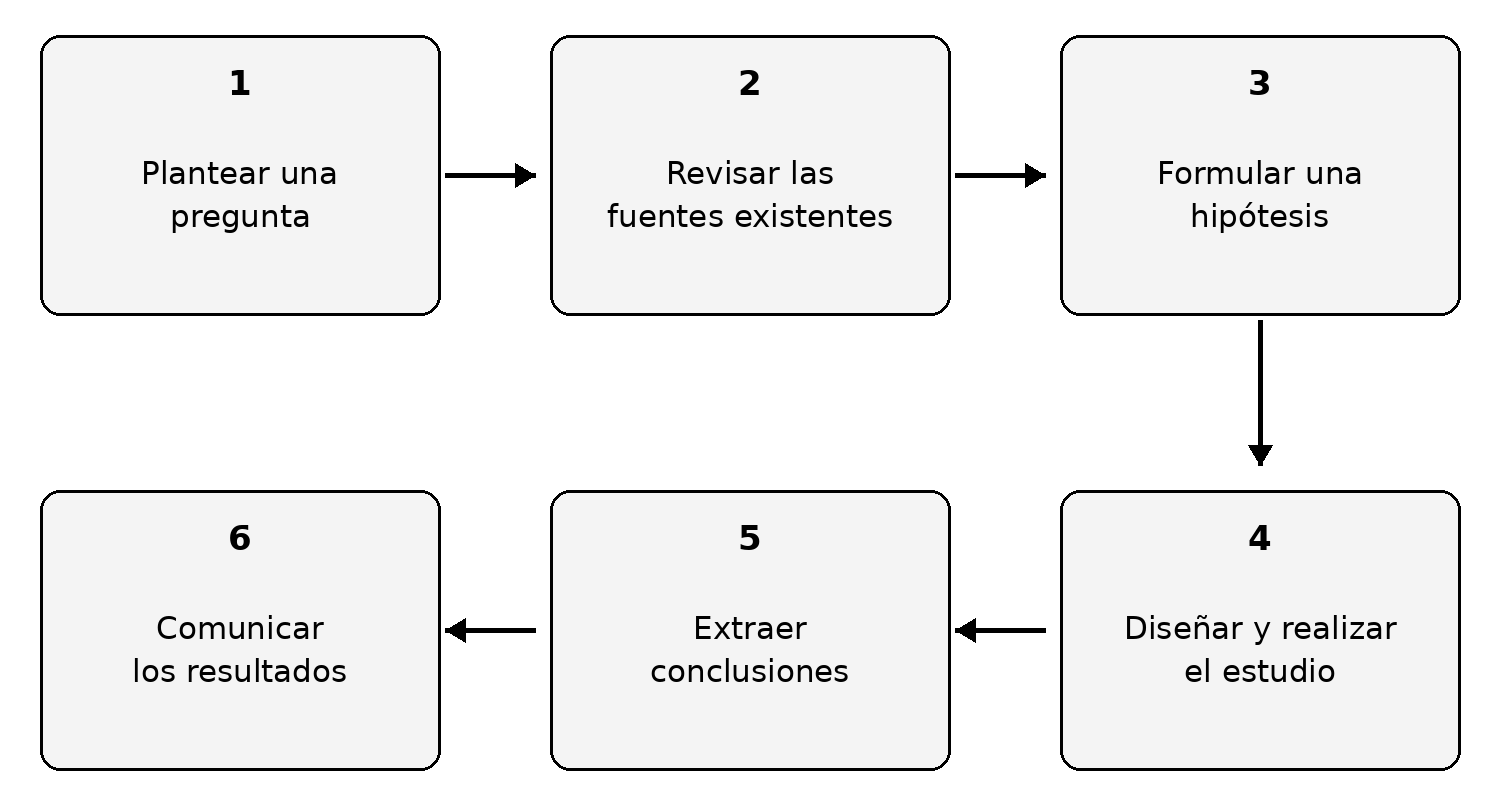
\includegraphics[width=\linewidth]{ITESCA/maestria-en-gestion-administrativa/seminario-i-mga/tarea6/fuentes/figura1-metodo-cientifico-es.png}
\apanota{\emph{Nota. }Traducida y redibujada a partir de la figura 2.2, “The Scientific Method”, en \emph{Introduction to Sociology 3e}, por T. R. Conerly, K. Holmes y A. L. Tamang, 2021, OpenStax (\url{https://openstax.org/books/introduction-sociology-3e/pages/2-1-approaches-to-sociological-research}). Copyright 2021 Rice University. Adaptación bajo CC BY-NC-SA 4.0 (\url{https://creativecommons.org/licenses/by-nc-sa/4.0/}).}
\end{minipage}
\end{figure}

\subsection{Aplicación del marco metodológico}

Detalla las estrategias específicas empleadas en el estudio.

\subsubsection{Tipo y diseño de estudio}

Indica si es experimental, no experimental, transversal o longitudinal.

\subsubsection{Población y muestra objeto de estudio}

Describe el universo y el tamaño de muestra seleccionada, justificando los criterios de inclusión.

\subsection{Instrumentos para recabar información}

Especifica los instrumentos de medición o técnicas utilizadas (encuestas, entrevistas, cuestionarios, observaciones, etc.), indicando su validez y confiabilidad.

La Figura 2 muestra un cuestionario en soporte digital, un ejemplo de instrumento para recabar información. El medio tecnológico no garantiza por sí mismo la validez: las preguntas deben corresponder a las variables y al propósito del estudio (Conerly et al., 2021).

\begin{figure}[H]
\begin{minipage}{\linewidth}
\caption{Aplicación de un cuestionario mediante una tableta}\label{fig:tarea6-2}
\centering
\includegraphics[width=0.82\linewidth]{ITESCA/maestria-en-gestion-administrativa/seminario-i-mga/tarea6/fuentes/figura2-cuestionario.png}
\apanota{\emph{Nota. }Reproducida de la figura 2.3 de \emph{Introduction to Sociology 3e}, por T. R. Conerly, K. Holmes y A. L. Tamang, 2021, OpenStax (\url{https://openstax.org/books/introduction-sociology-3e/pages/2-2-research-methods}). Crédito de la fotografía original: CDC Global/Flickr. Se conserva la atribución indicada en el libro; reutilización educativa no comercial conforme a su apartado “Art attribution” y licencia CC BY-NC-SA 4.0 (\url{https://creativecommons.org/licenses/by-nc-sa/4.0/}).}
\end{minipage}
\end{figure}

\subsection{Procedimiento para la obtención de datos}

Detalla las etapas y pasos seguidos para recolectar la información, así como los recursos, materiales y cronograma empleados.

\subsection{Plan de análisis de datos}

Describe cómo se procesarán los datos recolectados (análisis estadístico, categorización, codificación o triangulación), según el tipo de investigación.

\clearpage\section{Resultados y discusión}

Presenta los resultados obtenidos y su interpretación con base en los objetivos y el marco teórico.

\subsection{Aplicación de instrumentos y técnicas para la recolección de información}

Explica cómo se aplicaron los instrumentos, los contextos y las condiciones en que se desarrolló el trabajo de campo.

\subsection{Trabajo de campo}

Describe la experiencia práctica, las observaciones y los ajustes realizados durante la aplicación metodológica.

\subsection{Descripción de resultados preliminares}

Expone los principales hallazgos de manera objetiva, apoyándose en tablas, figuras o gráficos.

\subsection{Interpretación de resultados}

Analiza los resultados a la luz del marco teórico, estableciendo comparaciones con estudios previos o hipótesis planteadas.

\subsection{Principales hallazgos}

Resume los descubrimientos más relevantes y su contribución al conocimiento o a la solución del problema planteado.

\clearpage\section{Conclusiones y recomendaciones}

Integra los aportes finales del estudio y sugiere acciones o líneas futuras de investigación.

\subsection{Conclusiones}

Responde a los objetivos planteados, sintetizando los resultados más significativos.

\subsection{Recomendaciones}

Plantea sugerencias prácticas o teóricas para la mejora o continuidad del tema de estudio.

\subsection{Sugerencias para futuras investigaciones}

Propone posibles líneas de investigación o ampliaciones del estudio que puedan desarrollarse posteriormente.

\clearpage\section{Referencias bibliográficas}

Incluye todas las fuentes citadas en el trabajo, redactadas conforme al formato APA 7ª edición, con autores, año, título, editorial y enlace DOI o URL si aplica.

\begin{apareferences}

\item Conerly, T. R., Holmes, K., \& Tamang, A. L. (2021). \emph{Introduction to sociology 3e}. OpenStax. \url{https://openstax.org/details/books/introduction-sociology-3e}

\item \emph{Material para ejemplo}. (s. f.). [Material didáctico de Seminario I]. ITESCA Virtual. \url{https://cursos3.e-itesca.edu.mx/mod/assign/view.php?id=2889}

\item Organización de las Naciones Unidas. (1948). \emph{Declaración Universal de los Derechos Humanos}. \url{https://www.un.org/es/about-us/universal-declaration-of-human-rights}

\item Organización de las Naciones Unidas. (2015). \emph{Transformar nuestro mundo: La Agenda 2030 para el Desarrollo Sostenible}. \url{https://sdgs.un.org/es/2030agenda}

\item \emph{Resumen del Manual APA (7.ª edición): Aplicado al Seminario de Investigación y trabajos de titulación}. (s. f.). [Recurso 2.1 de Seminario I]. ITESCA Virtual. \url{https://cursos3.e-itesca.edu.mx/mod/url/view.php?id=2881}

\end{apareferences}

\clearpage\section{Anexos}

Reúne material complementario que respalda el trabajo (instrumentos aplicados, gráficas, reglamentos, encuestas, fotografías, etc.), cuya extensión impide incluirlos en el cuerpo principal.
